\documentclass{beamer}
\usepackage[T1]{fontenc}
\usepackage{bookman}
\usetheme[numbering=fraction, progressbar=foot, ,block=fill]{metropolis}  %source : https://fr.overleaf.com/latex/templates/metropolis-beamer-theme/qzyvdhrntfmr et https://mirror.foobar.to/CTAN/macros/latex/contrib/beamer-contrib/themes/metropolis/doc/metropolistheme.pdf

\usepackage{enumitem}
\usepackage{pifont} % puces des listes
\usepackage{blindtext}
\usepackage{hyperref}
\usepackage{fourier}  %symbole \danger
\usepackage[french]{babel}

%%%%%%%%%%%%%%%%%%%%%%%%%%%%%%%%%%%%%%%%%%%%%%%%%%%%%%%%%
%Information to be included in the title page:

\title{Ordonnance fédérale sur la Mensuration Officielle -- OMO}
\subtitle{Articles 29 \& 30}
\author{Maxime Fourquaux}
\institute[HEIG]%
{
    HEIG-VD  -- EC+G \\
    Orientation GGT
}
\date{Jeudi 31 mars 2022}
\logo{
\includegraphics[width=0.75cm]{picture/HEIG-VD_logotype_rouge-rvb.eps}}
%\logo{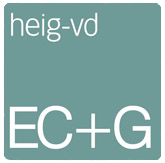
\includegraphics[width=0.75cm]{logoEC+G_163x165_ss_txt_ssBordBlanc.png}}

%%%%%%%%%%%%%%%%%%%%%%%%%%%%%%%%%%%%%%%%%%%%%%%%%%%%%%%%%




%%%%%%%%%%%%%%%%%%%%%%%%%%%%%%%%%%%%%%%%%%%%%%%%%%%%%%%%%
\renewcommand{\up}[1]{\textsuperscript{#1}}
\def\labelenumi{\theenumi}
\setbeamertemplate{enumerate item}{\alph{enumi}}
\setbeamertemplate{enumerate subitem}{\roman{enumii}.}
\usepackage{outline}%
\def\labeloutlni{\theoutlni}%
\def\theoutlni{\alph{outlni}.}%
%\renewcommand{\labelenumi}{\alph{enumi}.)

%\metroset{block=fill} %remplir les blocks

%%%%%%%%%%%%%%%%%%%%%%%%%%%%%%%%%%%%%%%%%%%%%%%%%%%%%%%%%
\begin{document}

\frame{\titlepage}

\begin{frame}
    \frametitle{OMO}
    Chapitre 4 -- Premier Relevé, renouvellement et mise à jour \\
    \bigskip
    Section 4 -- Procéduresuma d'opposition, approbation et indemnisation \\
    \bigskip
    \textbf{Articles 29 \& 30}
\end{frame}

\begin{frame}
    \frametitle{Présentation de l'article}
    \begin{alertblock}{Art. 29 -- Approbation}
        \up{1} Au terme de l’enquête publique et après le règlement des oppositions formées auprès de la première instance, \alert{l’autorité cantonale compétente approuve}, indépendamment des litiges à régler par voie judiciaire, \alert {les données de la mensuration officielle} et les extraits produits sur cette base, notamment le plan du registre foncier, dès lors : \pause
        \begin{outline}
            \item que les données répondent aux exigences qualitatives et techniques prévues par le droit fédéral; \pause
            \item qu’un éventuel examen préalable a donné un résultat favorable, et \pause
            \item que les défauts relevés par un examen préalable ont été corrigés
        \end{outline}
    \end{alertblock}
\end{frame}

\begin{frame}
    \frametitle{Mise en application -- Art. 29, al. 1}
    \textbf{(VD)} Art. 30, al. 1, LGéo-VD : Département approuve \& publication dans la Feuille des avis officiels
    \bigskip
    \begin{figure}
        \centering
        
\includegraphics[scale=0.5]{picture/132LausanneApprobationOfficielleMensuration.png}
        %\caption{Caption}
        %\label{fig:my_label}
        \textit{Feuille des avis officiels (faovd.ch)}
    \end{figure} \pause
    \textbf{(GE)} Art. 24, al. 2, RMOC : Conseil d'Etat approuve \& publication dans la Feuille d'avis officielle
\end{frame}


\begin{frame}
    \frametitle{Présentation de l'article}
    \begin{alertblock}{Art. 29 -- Approbation}
        \up{2} L’approbation confère à ces \alert{éléments de la mensuration} le caractère de \alert{documents officiels}.
    \end{alertblock}
\end{frame}

\begin{frame}
    \frametitle{Mise en application -- Art. 29, al. 2}
    %\begin{exampleblock}{Art 30 Approbation et mise en vigueur (LGéo-VD) }
    %\up{1} (...) La reconnaissance de l'autorité fédérale est alors demandée.
    %\end{exampleblock}
    %\bigskip \pause
    \begin{exampleblock}{Art. 5 Documents officiels (LTrans, CH)}
        \up{1} On entend par document officiel toute information:
        \begin{outline}
            \item qui a été enregistrée sur un quelconque support;
            \item qui est détenue par l'autorité dont elle émane (...)
            \item qui concerne l'accomplissement d'une tâche publique.
        \end{outline}
    \end{exampleblock}
    \bigskip \pause
    \begin{exampleblock}{Art. 6 Principe de la transparence (LTrans, CH)}
        \up{1} Toute personne a le droit de consulter des documents officiels et d’obtenir des renseignements sur leur contenu de la part des autorités.
    \end{exampleblock}
\end{frame}

\begin{frame}
    \frametitle{Mise en application -- Art. 29, al. 2}
    \begin{exampleblock}{Art. 43, Mise en vigueur provisoire (LCMO, NE)}
        Le  service  peut  mettre  en  vigueur  les  documents  de  la  nouvelle mensuration au fur et à mesure de leur achèvement, sous réserve du résultat de l'enquête publique.
    \end{exampleblock}

    %\bigskip \pause
    %\begin{exampleblock}{Art. 61 Mise à l'enquête -- Publications (LMO, FR)}
    %\up{3} Les personnes dont l'adresse ne peut être obtenue ni auprès de l'administration communale, ni auprès du service chargé de la tenue du registre foncier ou du service chargé de l'administration des impôts directs sont réputées avisées par la publication faite dans la Feuille officielle.
    %\end{exampleblock}

    %\begin{itemize}[label=\ding{228}]
    %\item Demande de documents officiels sur : \href{https://www.swisstopo.admin.ch/fr/swisstopo/access.html}{www.swisstopo.admin.ch} \\ \textit{(Art 1, LTrans \\
    %\small Loi fédérale sur le principe de la transparence dans l'administration)}
    %\end{itemize}
\end{frame}

\begin{frame}
    \frametitle{Présentation de l'article}
    \begin{alertblock}{Art. 30 -- Reconnaissance par la Confédération}
        La Direction fédérale des mensurations cadastrales \alert{reconnaît les travaux de mensuration} lorsque : \pause
        \begin{outline}
            \item les données répondent aux \alert{exigences qualitatives et techniques} prévues par le droit  fédéral, et que \pause
            \item les travaux de mensuration ont été \alert{approuvés par le canton}.
        \end{outline}
    \end{alertblock}
\end{frame}

\begin{frame}
    \frametitle{Mise en application -- Article 30}
    \begin{itemize}[label=\ding{228}]
        \item Respect de l'art. 29, al. 1, let. a OMO ? \pause
        \item Approbation du canton ? \pause
    \end{itemize}
    $\Longrightarrow$ Approbation par la D+M
    %\pause \\
    %\bigskip
    %\warning ~ \href{https://www.fedlex.admin.ch/eli/cc/1994/1864_1864_1864/fr#art_109}{Art. 109, al. 1 OTEMO} : documents à transmettre en vue d'une reconnaissance
\end{frame}

\begin{frame}
    \frametitle{Transmission des documents}
    \begin{alertblock}{Art 109, OTEMO}
        \up{1} \footnotesize En vue de la reconnaissance visée à l’art. 30 OMO, \alert{les documents suivants doivent être remis à la Direction fédérale des mensurations cadastrales}: \pause
        \begin{outline}
            \item la demande de reconnaissance; \pause
            \item au besoin, une attestation confirmant l’élimination des défauts relevés lors de l’examen préalable visé à l’art. 27 OMO; \pause
            \item tous les documents de l’approbation cantonale, y compris le rapport du service cantonal du cadastre relatif à l’exécution et à la vérification de la mensuration officielle; \pause
            \item le procès-verbal de contrôle des données dressé par un service de contrôle désigné par la Direction fédérale des mensurations cadastrales, attestant que les données de la mensuration officielle sont disponibles dans le modèle de données de la Confédération et exemptes de toute erreur formelle; \pause
            \item le décompte final.
        \end{outline}
    \end{alertblock}
\end{frame}

\begin{frame}
    \frametitle{Transmission des documents}
    \begin{alertblock}{Art 109, OTEMO}
        \up{2} La Direction fédérale des mensurations cadastrales peut stipuler dans la convention-programme conclue avec le canton que d’autres documents et données doivent être fournis.
    \end{alertblock}
\end{frame}

\end{document}